\documentclass[lettersize,journal]{IEEEtran}
\usepackage{amsmath,amsfonts}
\usepackage{algorithmic}
\usepackage{algorithm}
\usepackage{array}
\usepackage[caption=false,font=normalsize,labelfont=sf,textfont=sf]{subfig}
\usepackage{textcomp}
\usepackage{stfloats}
\usepackage{url}
\usepackage{verbatim}
\usepackage{graphicx}
\usepackage{cite}
\usepackage{float}
\hyphenation{op-tical net-works semi-conduc-tor IEEE-Xplore}

\begin{document}

\title{CSC360 Final Project: Insertion Sort and Binary Search Algorithm Implementation in RISC-V Assembly}

\author{Mark Stotzer*, Dawson Blakeslee** \\ Hamm School of Engineering at the University of Mary, Bismarck, ND \\ *mpstotzer1@umary.edu, **diblakeslee1@umary.edu}

% The paper headers
\markboth{Paper for Professor Hayes' Course, \textit{CSC360: Computer Architecture}, April 15, 2026}%
{}

\maketitle

\begin{abstract}
\end{abstract}

\begin{IEEEkeywords}
\end{IEEEkeywords}

\section{Introduction}
\IEEEPARstart{H}{ere} is an example of how to cite\cite{ref1}.

\section{Background and Scope of Problem}
\indent 

\section{Design Approach}
\indent
	\subsection{Insertion Sort}
\indent The design process for the insertion sort algorithm began with research into how the algorithm functioned, as to best understand the problem, solution, and implementation. Next, a high-level flowchart was developed from the methods found during the research stage, and can be found in Figure \ref{insertion-high-flow}. From there, C code was made to accomplish the insertion sort task, which could then be more easily translated to RISC-V assembly. After the C implementation, a low-level flowchart (Figure \ref{insertion-low-flow}) was created, which proved very useful in the proceeding step-by-step translation into assembly. After the translation to assembly, the program was tested in Ripes to verify completeness and to observe certain metrics provided by Ripes. The C program was then translated once again into assembly, but this time using an optimized 'gcc' style compiler. Finally, the optimized compiler program was compared to the hand-generated program in Ripes to document improvements in CPI, clock cycles, instruction count, and execution time. 
	\subsection{Binary Search}
    For simple algorithms like binary search, the first step was drawing a high-level flowchart (see figure \ref{fig:highBinary}). Then, it was converted into C code and tested for bugs. This was converted into a low-level flowchart (figure \ref{fig:lowBinary}) and then, given the simplicity of the algorithm, converted into assembly by hand to produce the naive implementation. An optimized compiler-generated algorithm, referred to as just the compiler algorithm, followed, and both were tested in Ripes. Finally, after studying the hazards, they were modified into one final algorithm, called the modified algorithm.

    The algorithms were tested by averaging the cycles it took to find an element in the deepest level of the tree and two deepest level searches for items not in the tree (too low and too high, respectively). This produced the results seen in figure \ref{fig:clockCycles}.


\section{Flowcharts and Design Progression}
\indent 
	\subsection{Insertion Sort}
		\begin{figure}[H]
			\centering
			\includegraphics[width=0.75\linewidth]{./../insertion-sort/Figures/high-level.png}
				\caption{High-Level Insertion Sort Flowchart}
				\label{insertion-high-flow}
		\end{figure}
		\begin{figure}[H]
			\centering
			\includegraphics[width=0.75\linewidth]{./../insertion-sort/Figures/low-level.png}
				\caption{Low-Level Insertion Sort Flowchart}
				\label{insertion-low-flow}
		\end{figure}

	\subsection{Binary Search}
    
    \begin{figure}[H]
        \centering
        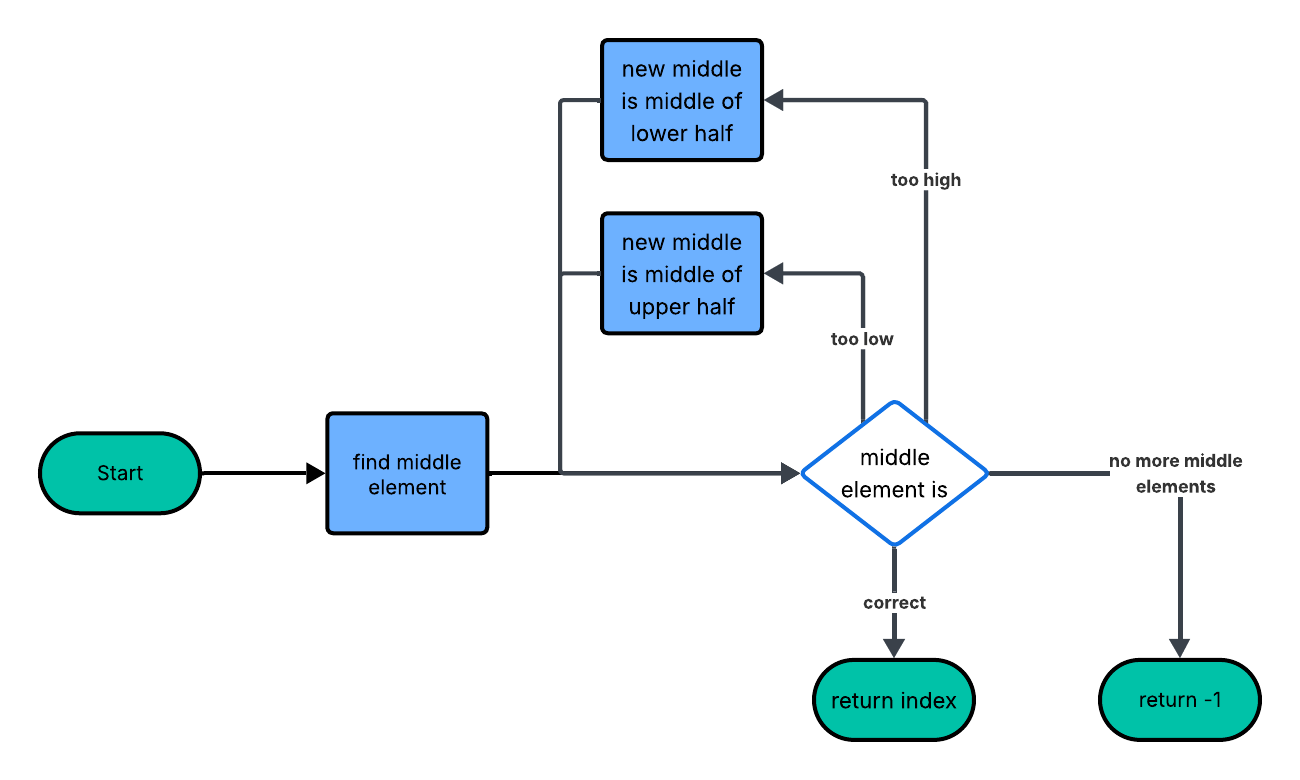
\includegraphics[width=0.75\linewidth]{./../binary-search/Figures/BinarySearchHigh.png}
        \caption{High-Level Binary Search Flowchart}
        \label{fig:highBinary}
    \end{figure}
    
    \begin{figure}[H]
        \centering
        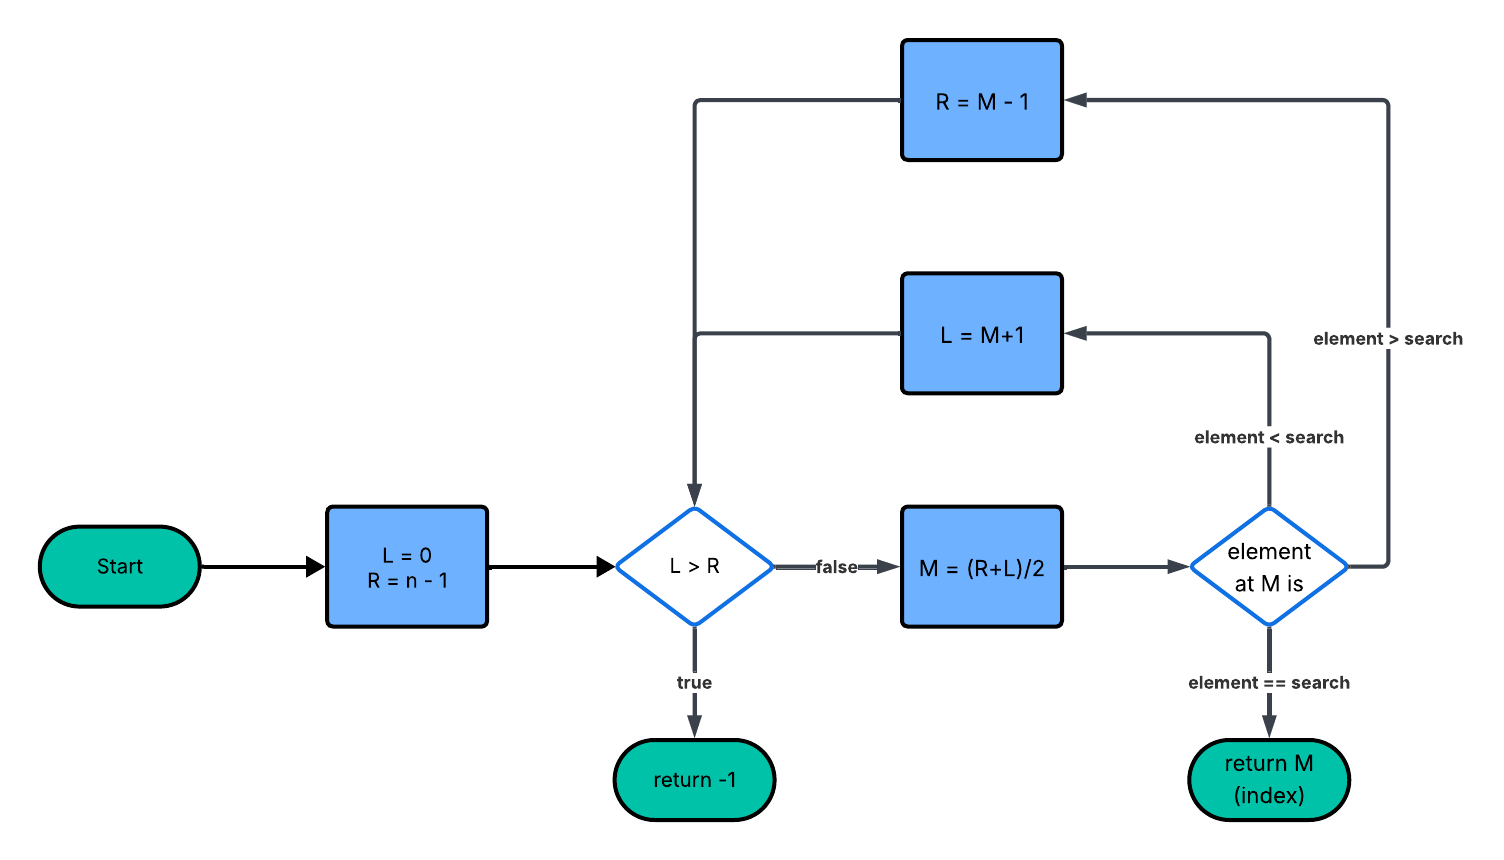
\includegraphics[width=0.75\linewidth]{./../binary-search/Figures/BinarySearchLow.png}
        \caption{Low-Level Binary Search Flowchart}
        \label{fig:lowBinary}
    \end{figure}

    \begin{figure}[H]
        \centering
        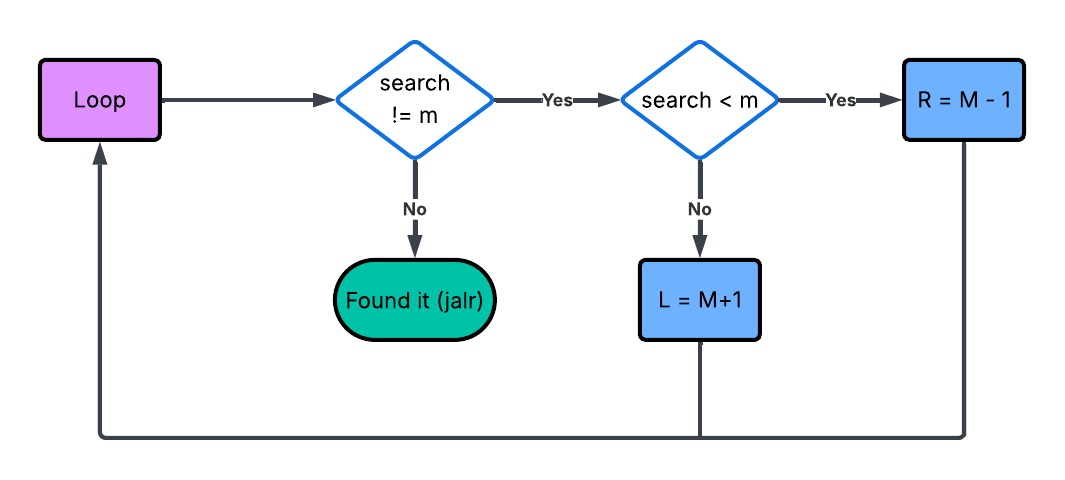
\includegraphics[width=0.75\linewidth]{./../binary-search/Figures/NonPipelinedBranching.png}
        \caption{Non-Pipelined Naive Branching}
        \label{fig:naiveBranching}
    \end{figure}

    \begin{figure}[H]
        \centering
        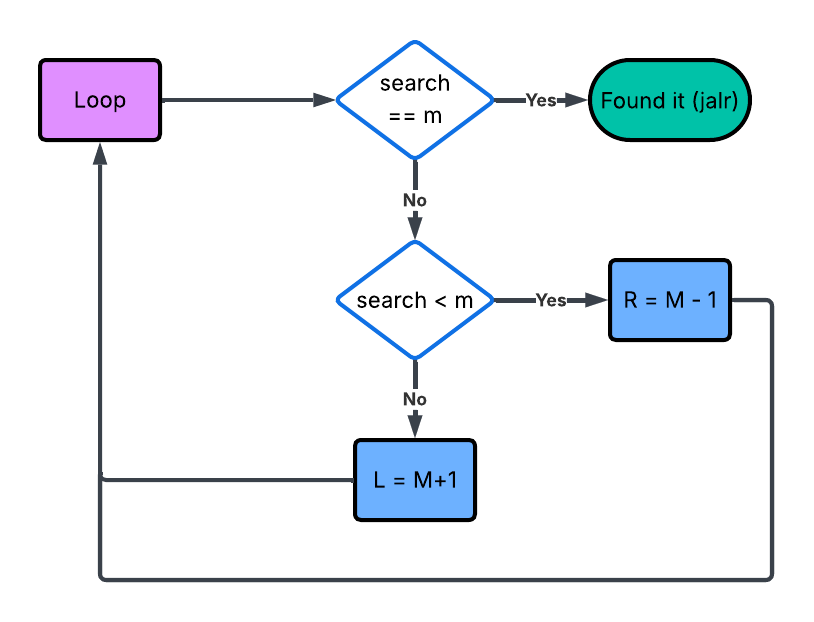
\includegraphics[width=0.75\linewidth]{./../binary-search/Figures/PipelinedBranching.png}
        \caption{Pipelined Modified Branching}
        \label{fig:modifiedBranching}
    \end{figure}
    
\section{Pipelining and Hazards}
\indent 
	\subsection{Insertion Sort}
	\subsection{Binary Search}
    Looking at the different algorithm diagrams, there are two hazards. First is a load-use hazard "lw x31, 0, x31" followed by a branch statement using x31. This is common to all three since the code could not be rearranged to place this earlier.

    The second hazard is a branch hazard rooted in the arrangement of branch statements in the assembly code. In the naive algorithm (Fig. \ref{fig:naiveBranching}), one branch statement jumped to the next upon success in a daisy chain pattern. This caused the two pipelined instructions after to be flushed upon failure. Since there were three cases, the chance of any branch failing was higher than those of it succeeding. There was an opportunity for three branch hazards per loop. Both the modified and compiler algorithms prevented this by placing all branch statements adjecent to each other in the code (see Fig. \ref{fig:modifiedBranching}). As such, a failure would fall through to evaluating the next branch, causing at most one branch hazard per loop.
    

\section{Assembly Implementation}
\indent 
	\subsection{Insertion Sort}
	\subsection{Binary Search}
    There were three different assembly implementations: the naive, the compiler, and the modified. The naive and modified are entirely the same except for the order of branching (see section V for details). The compiler version has the same branch ordering trick as the modified, but included two few extra instructions on top. First, it set the return register to -1 by default, saving a cycle later if the item was not found but wasting a cycle if it was. Second, it immediately checked if the array length was greater than zero, saving time for an invalid array parameter but wasting time on valid ones.

    \begin{figure}[H]
        \centering
        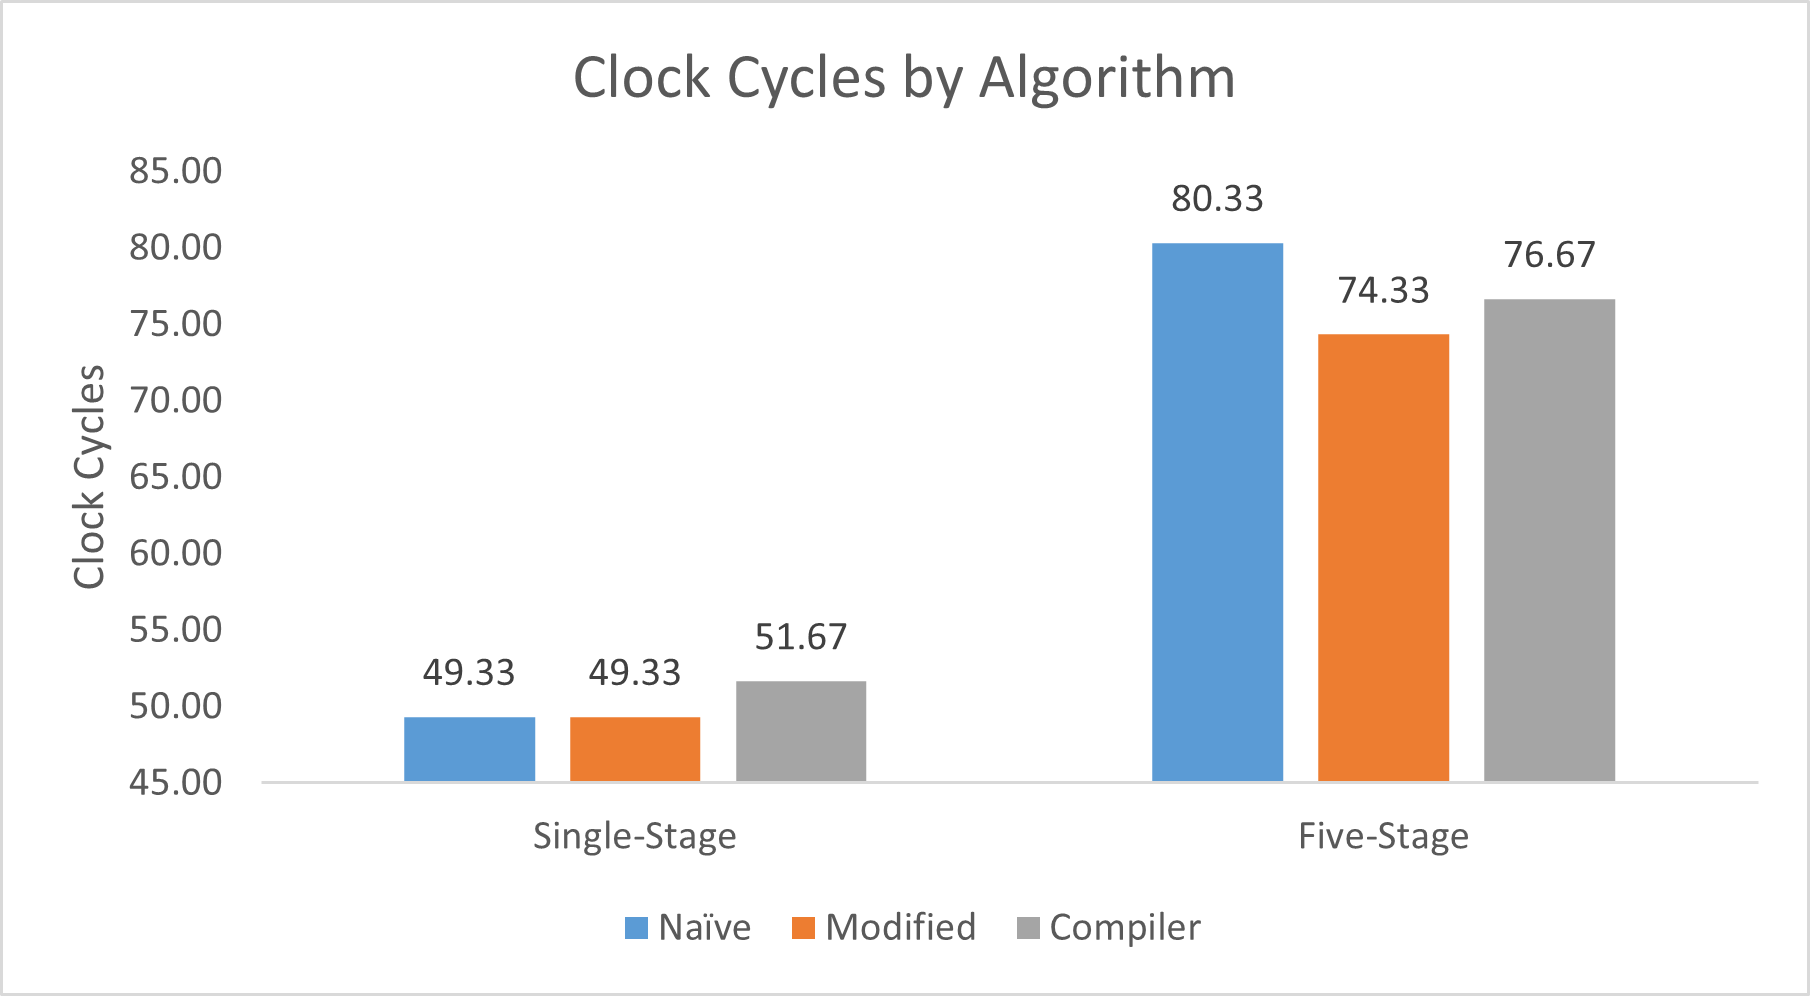
\includegraphics[width=0.75\linewidth]{./../binary-search/Figures/ClockCyclesByAlgorithm.png}
        \caption{Performance by Algorithm and Processor}
        \label{fig:clockCycles}
    \end{figure}

    \begin{figure}[H]
        \centering
        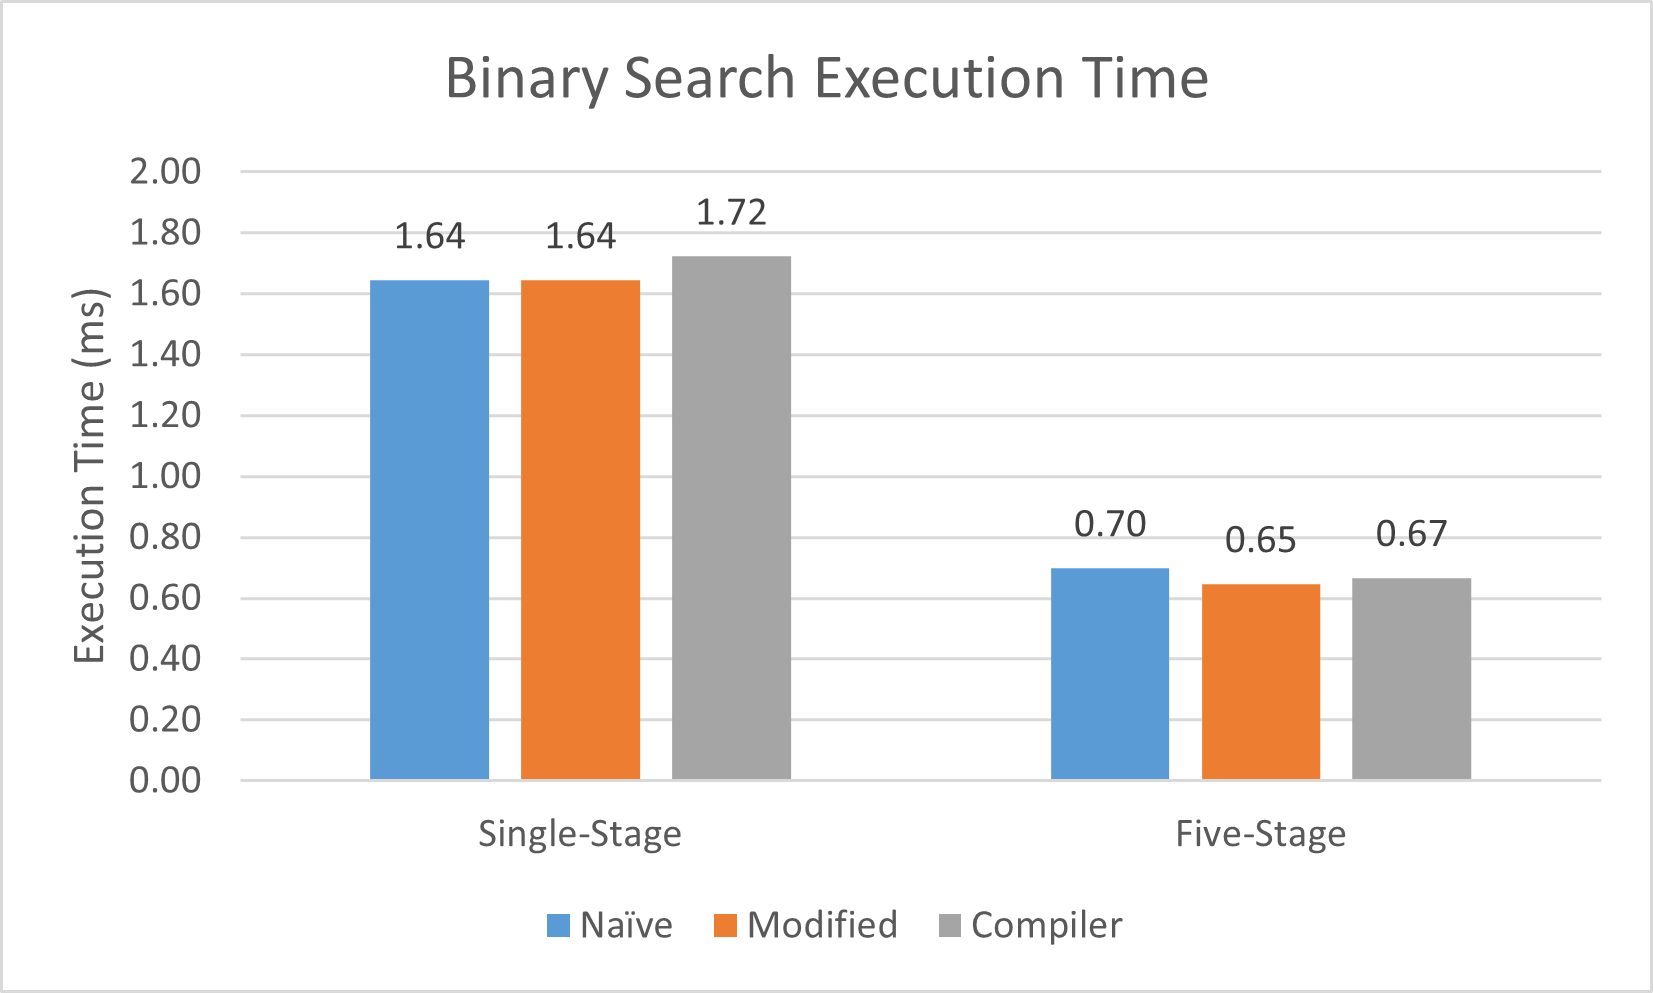
\includegraphics[width=0.75\linewidth]{./../binary-search/Figures/executionTimeByAlgorithm.png}
        \caption{Execution Time by Algorithm and Processor}
        \label{fig:executionTime}
    \end{figure}
    
    

\section{Results}
\indent 
	\subsection{Insertion Sort}
	\subsection{Binary Search}
    The fastest algorithm, for both processors, was the modified algorithm. It tied with the naive in single-stage, given that there is no branch penalty, and beat the compiler by approximately two cycles. In the five-stage, the branch arrangement for modified and compiler easily beat out naive. Still, the compiler's extra introductory steps served to slow it down by 2 cycles.

    It should be noted that single stage took half the cycles of five-stage, because the latter must flush and stall frequently. However, the advantage is that the five-stage runs five cycles in the time the single-stage runs one. In practice, due to added hardware complexity for pipelining, the clock period is only around three times as fast. A standard clock period for RISC-V hardware was found online: 30 and 115 MHz for single and five-stage respectively. The estimated execution times, seen in figure \ref{fig:executionTime}, demonstrate the same pattern identified above: modified is fastest. 

\section{Conclusion}
\indent 

\begin{thebibliography}{1}
\bibliographystyle{IEEEtran}

\bibitem{ref1}

\bibitem{ref2}

\end{thebibliography}

\newpage

\vfill

\end{document}
